\documentclass{standalone}
\usepackage{tikz}
\usetikzlibrary{patterns, positioning}


\begin{document}
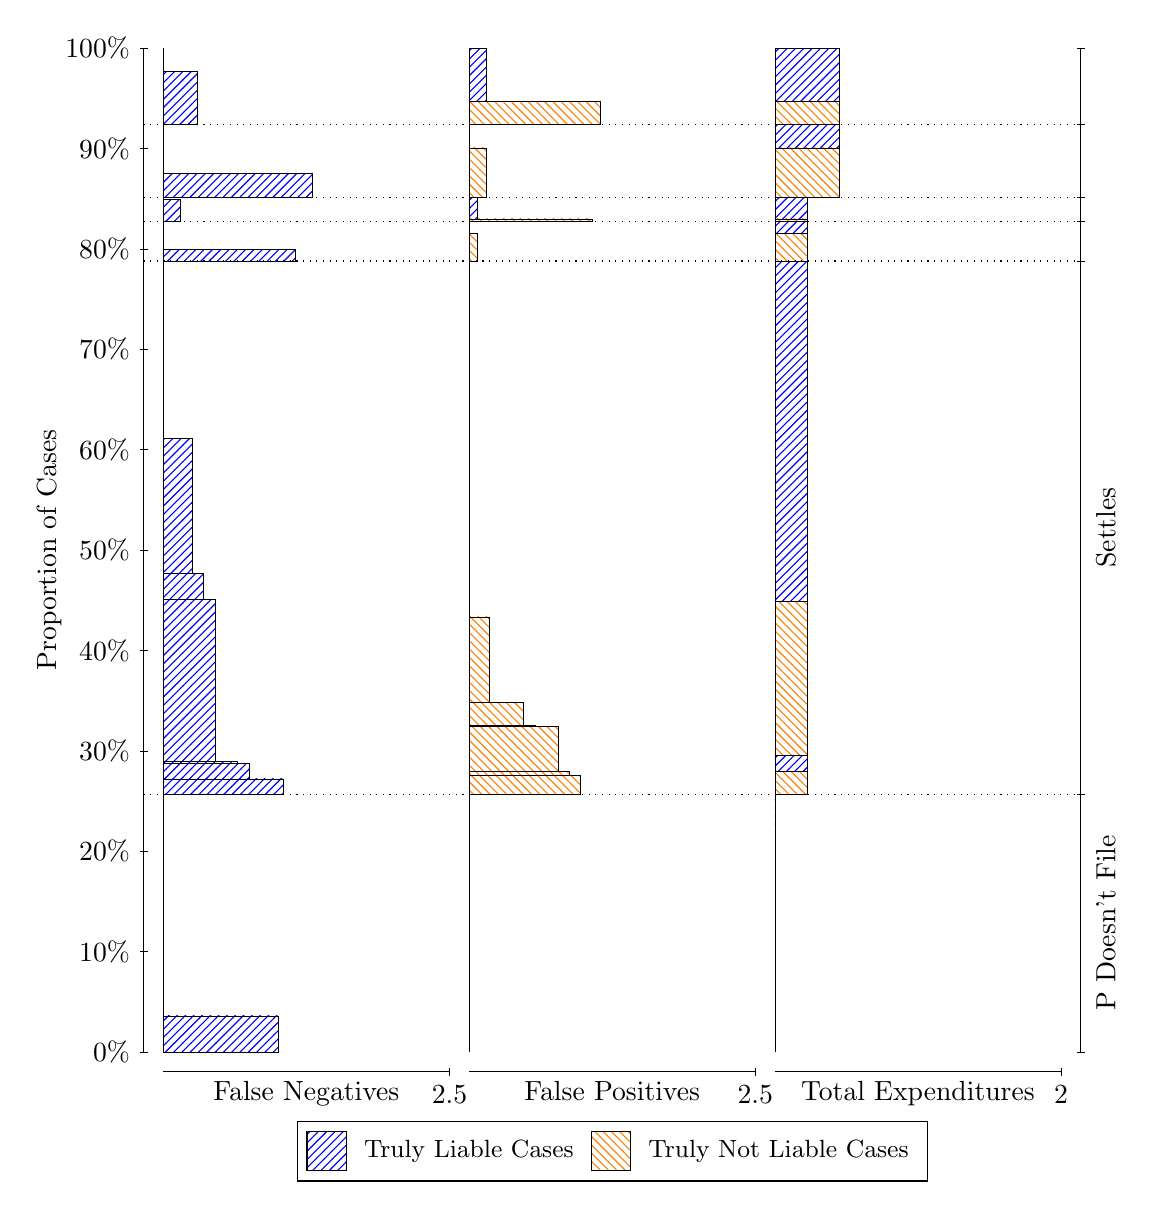
\begin{tikzpicture}
\draw[black, very thin] (1.5,1.75) -- (1.5,14.5);
\node[rotate=90, text=black, anchor=center] at (0.3, 8.125) {Proportion of Cases};
\draw[black, very thin] (1.45,1.75) -- (1.55,1.75);
\node[text=black, anchor=east] at (1.45, 1.75) {0\%};
\draw[black, very thin] (1.45,3.025) -- (1.55,3.025);
\node[text=black, anchor=east] at (1.45, 3.025) {10\%};
\draw[black, very thin] (1.45,4.3) -- (1.55,4.3);
\node[text=black, anchor=east] at (1.45, 4.3) {20\%};
\draw[black, very thin] (1.45,5.575) -- (1.55,5.575);
\node[text=black, anchor=east] at (1.45, 5.575) {30\%};
\draw[black, very thin] (1.45,6.85) -- (1.55,6.85);
\node[text=black, anchor=east] at (1.45, 6.85) {40\%};
\draw[black, very thin] (1.45,8.125) -- (1.55,8.125);
\node[text=black, anchor=east] at (1.45, 8.125) {50\%};
\draw[black, very thin] (1.45,9.4) -- (1.55,9.4);
\node[text=black, anchor=east] at (1.45, 9.4) {60\%};
\draw[black, very thin] (1.45,10.675) -- (1.55,10.675);
\node[text=black, anchor=east] at (1.45, 10.675) {70\%};
\draw[black, very thin] (1.45,11.95) -- (1.55,11.95);
\node[text=black, anchor=east] at (1.45, 11.95) {80\%};
\draw[black, very thin] (1.45,13.225) -- (1.55,13.225);
\node[text=black, anchor=east] at (1.45, 13.225) {90\%};
\draw[black, very thin] (1.45,14.5) -- (1.55,14.5);
\node[text=black, anchor=east] at (1.45, 14.5) {100\%};

\draw[black, very thin] (13.4,1.75) -- (13.4,14.5);
\draw[black, very thin] (13.35,1.75) -- (13.45,1.75);
\node[anchor=west] at (13.35, 1.75) {};
\draw[black, very thin] (13.35,5.0251) -- (13.45,5.0251);
\node[anchor=west] at (13.35, 5.0251) {};
\draw[black, very thin] (13.35,11.795) -- (13.45,11.795);
\node[anchor=west] at (13.35, 11.795) {};
\draw[black, very thin] (13.35,12.298) -- (13.45,12.298);
\node[anchor=west] at (13.35, 12.298) {};
\draw[black, very thin] (13.35,12.607) -- (13.45,12.607);
\node[anchor=west] at (13.35, 12.607) {};
\draw[black, very thin] (13.35,13.53) -- (13.45,13.53);
\node[anchor=west] at (13.35, 13.53) {};
\draw[black, very thin] (13.35,14.5) -- (13.45,14.5);
\node[anchor=west] at (13.35, 14.5) {};

\draw[black, very thin, pattern color=blue, pattern=north east lines] (1.75,1.75) rectangle (3.2033,2.2079);
\draw[black, very thin, pattern color=orange, pattern=north west lines] (1.75,2.2079) rectangle (1.75,5.0251);
\draw[black, very thin, pattern color=blue, pattern=north east lines] (1.75,5.0251) rectangle (3.276,5.2195);
\draw[black, very thin, pattern color=blue, pattern=north east lines] (1.75,5.2195) rectangle (2.84,5.4169);
\draw[black, very thin, pattern color=blue, pattern=north east lines] (1.75,5.4169) rectangle (2.6947,5.4416);
\draw[black, very thin, pattern color=blue, pattern=north east lines] (1.75,5.4416) rectangle (2.404,7.4935);
\draw[black, very thin, pattern color=blue, pattern=north east lines] (1.75,7.4935) rectangle (2.2587,7.8294);
\draw[black, very thin, pattern color=blue, pattern=north east lines] (1.75,7.8294) rectangle (2.1133,9.545);
\draw[black, very thin, pattern color=orange, pattern=north west lines] (1.75,9.545) rectangle (1.75,11.795);
\draw[black, very thin, pattern color=blue, pattern=north east lines] (1.75,11.795) rectangle (3.4213,11.946);
\draw[black, very thin, pattern color=orange, pattern=north west lines] (1.75,11.946) rectangle (1.75,12.298);
\draw[black, very thin, pattern color=blue, pattern=north east lines] (1.75,12.298) rectangle (1.968,12.573);
\draw[black, very thin, pattern color=orange, pattern=north west lines] (1.75,12.573) rectangle (1.75,12.607);
\draw[black, very thin, pattern color=blue, pattern=north east lines] (1.75,12.607) rectangle (3.6393,12.904);
\draw[black, very thin, pattern color=orange, pattern=north west lines] (1.75,12.904) rectangle (1.75,13.53);
\draw[black, very thin, pattern color=blue, pattern=north east lines] (1.75,13.53) rectangle (2.186,14.202);
\draw[black, very thin, pattern color=orange, pattern=north west lines] (1.75,14.202) rectangle (1.75,14.5);
\draw[black, very thin, pattern color=orange, pattern=north west lines] (5.6333,1.75) rectangle (5.6333,4.5672);
\draw[black, very thin, pattern color=blue, pattern=north east lines] (5.6333,4.5672) rectangle (5.6333,5.0251);
\draw[black, very thin, pattern color=orange, pattern=north west lines] (5.6333,5.0251) rectangle (7.0503,5.2664);
\draw[black, very thin, pattern color=orange, pattern=north west lines] (5.6333,5.2664) rectangle (6.905,5.3176);
\draw[black, very thin, pattern color=orange, pattern=north west lines] (5.6333,5.3176) rectangle (6.7597,5.8861);
\draw[black, very thin, pattern color=orange, pattern=north west lines] (5.6333,5.8861) rectangle (6.469,5.8991);
\draw[black, very thin, pattern color=orange, pattern=north west lines] (5.6333,5.8991) rectangle (6.3237,6.1909);
\draw[black, very thin, pattern color=orange, pattern=north west lines] (5.6333,6.1909) rectangle (5.8877,7.2749);
\draw[black, very thin, pattern color=blue, pattern=north east lines] (5.6333,7.2749) rectangle (5.6333,11.795);
\draw[black, very thin, pattern color=orange, pattern=north west lines] (5.6333,11.795) rectangle (5.7423,12.146);
\draw[black, very thin, pattern color=blue, pattern=north east lines] (5.6333,12.146) rectangle (5.6333,12.298);
\draw[black, very thin, pattern color=orange, pattern=north west lines] (5.6333,12.298) rectangle (7.1957,12.331);
\draw[black, very thin, pattern color=blue, pattern=north east lines] (5.6333,12.331) rectangle (5.7423,12.607);
\draw[black, very thin, pattern color=orange, pattern=north west lines] (5.6333,12.607) rectangle (5.8513,13.232);
\draw[black, very thin, pattern color=blue, pattern=north east lines] (5.6333,13.232) rectangle (5.6333,13.53);
\draw[black, very thin, pattern color=orange, pattern=north west lines] (5.6333,13.53) rectangle (7.3047,13.827);
\draw[black, very thin, pattern color=blue, pattern=north east lines] (5.6333,13.827) rectangle (5.8513,14.5);
\draw[black, very thin, pattern color=orange, pattern=north west lines] (9.5167,1.75) rectangle (9.5167,4.5672);
\draw[black, very thin, pattern color=blue, pattern=north east lines] (9.5167,4.5672) rectangle (9.5167,5.0251);
\draw[black, very thin, pattern color=orange, pattern=north west lines] (9.5167,5.0251) rectangle (9.9254,5.3168);
\draw[black, very thin, pattern color=blue, pattern=north east lines] (9.5167,5.3168) rectangle (9.9254,5.5143);
\draw[black, very thin, pattern color=orange, pattern=north west lines] (9.5167,5.5143) rectangle (9.9254,7.4723);
\draw[black, very thin, pattern color=blue, pattern=north east lines] (9.5167,7.4723) rectangle (9.9254,11.795);
\draw[black, very thin, pattern color=orange, pattern=north west lines] (9.5167,11.795) rectangle (9.9254,12.146);
\draw[black, very thin, pattern color=blue, pattern=north east lines] (9.5167,12.146) rectangle (9.9254,12.298);
\draw[black, very thin, pattern color=orange, pattern=north west lines] (9.5167,12.298) rectangle (9.9254,12.331);
\draw[black, very thin, pattern color=blue, pattern=north east lines] (9.5167,12.331) rectangle (9.9254,12.607);
\draw[black, very thin, pattern color=orange, pattern=north west lines] (9.5167,12.607) rectangle (10.334,13.232);
\draw[black, very thin, pattern color=blue, pattern=north east lines] (9.5167,13.232) rectangle (10.334,13.53);
\draw[black, very thin, pattern color=orange, pattern=north west lines] (9.5167,13.53) rectangle (10.334,13.827);
\draw[black, very thin, pattern color=blue, pattern=north east lines] (9.5167,13.827) rectangle (10.334,14.5);
\draw[black, dotted] (1.5,5.0251) -- (13.4,5.0251);
\draw[black, dotted] (1.5,11.795) -- (13.4,11.795);
\draw[black, dotted] (1.5,12.298) -- (13.4,12.298);
\draw[black, dotted] (1.5,12.607) -- (13.4,12.607);
\draw[black, dotted] (1.5,13.53) -- (13.4,13.53);
\draw[black, very thin] (1.75,1.5) -- (5.3833,1.5);
\node[text=black, anchor=north] at (3.5667, 1.5) {False Negatives};
\draw[black, very thin] (5.3833,1.45) -- (5.3833,1.55);
\node[text=black, anchor=north] at (5.3833, 1.45) {2.5};

\draw[black, very thin] (5.6333,1.5) -- (9.2667,1.5);
\node[text=black, anchor=north] at (7.45, 1.5) {False Positives};
\draw[black, very thin] (9.2667,1.45) -- (9.2667,1.55);
\node[text=black, anchor=north] at (9.2667, 1.45) {2.5};

\draw[black, very thin] (9.5167,1.5) -- (13.15,1.5);
\node[text=black, anchor=north] at (11.333, 1.5) {Total Expenditures};
\draw[black, very thin] (13.15,1.45) -- (13.15,1.55);
\node[text=black, anchor=north] at (13.15, 1.45) {2};

\node[text=black, centered, rotate=90] at (13.72, 3.3875) {P Doesn't File};
\node[text=black, centered, rotate=90] at (13.72, 8.4099) {Settles};





\draw (7.449999999999999,1.5) node[draw=none] (baseCoordinate) {};
\begin{scope}[align=center]
        \matrix[scale=0.5, draw=black, below=0.5cm of baseCoordinate, nodes={draw}, column sep=0.1cm]{
            \node[rectangle, draw, minimum width=0.5cm, minimum height=0.5cm, pattern color=blue, pattern=north east lines] {}; &
            \node[draw=none, font=\small, text=black] (B) {Truly Liable Cases}; &
            \node[rectangle, draw, minimum width=0.5cm, minimum height=0.5cm, pattern color=orange, pattern=north west lines] {}; &
            \node[draw=none, font=\small, text=black] (B) {Truly Not Liable Cases}; \\
            };
\end{scope}

\end{tikzpicture}
\end{document}